\chapter{Foundations}\label{foundations}
Most of the groundwork of the methods we will be using was invented in the second half of the 20th century. They include reinforcement learning---a general framework defining the aim of the playing algorithm, Q-learning---a simple algorithm to learn to play a game, and basics of neural networks---the statistical model that was used to overcome Q-learning's limitations.
This foundation work, joined with the recent (after $2010$) advances in the methods of training and architectures of neural networks allowed to vastly improve the former results.

This chapter discusses these methods, as well as describes the Atari machine, as the games we are interested in playing are created for this platform.

\section{Reinforcement learning}
To create an algorithm learning to play a game or solve any other problem, we first have to formally define what the problem is. We will model Atari games within the framework called reinforcement learning. The main property distinguising reinforcement learning problems from supervised learning (prediction) and unsupervised learning (clustering) is presence of two separate entities: the \emph{environment} and the \emph{agent}.

The environment is the physics or the rules of the game. It presents state, which can be any description of the game, to the agent, scores its action and provides him with the following state.
The agent is the algorithm we prepare. It receives a state it is in from the environment, decides which action to choose there and receives the appropriate reward. Every move happens in a discrete moments of time.

The aim of the creator of the reinforcement learning algorithm is to invent a way to map the game state for each time $t$: $s_t$ to the action $a_t$ (possibly storing some inner state), so that the sum:
\begin{equation} \label{discounted-reward}
\sum_{k=0}^{\infty} \gamma^k r_{t + k}
\end{equation}
is maximized.  $r_T$ is the reward received after doing action $a_T$ in state $s_T$ The exponential averaging is called a \emph{discounted} sum, and $0 < \gamma \le 1$ is called a \emph{discount factor} corresponds to the level of comfort we have with receiving the awards not now, but in the future. This resembles the way people evaluate their gains---if one is promissed a constant amount of money, he'd prefer to receive it rather earlier than later.

Both agent and environment are not bound to make their decisions deterministically---in fact, it may be favorable for the agent to play randomly to some extent. In the stochastic case, the aim of the agent is to maximize the discounted sum of expected value of the rewards.

\begin{figure}[!h]
  \center
  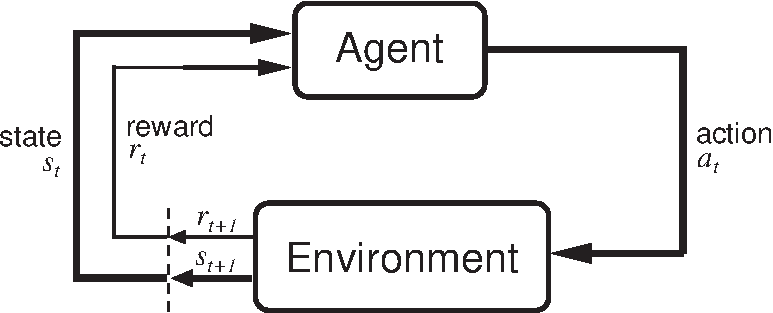
\includegraphics[scale=0.8]{images/Agent-Env-crop.pdf}
  \caption{The interaction between the agent and the environment, from \cite{reinforcement-book}.}
\end{figure}

The reinforcement learning, as defined above is a very general framework which can describe a broad range of problems. To make it easier to model it using statistical tools, we assume all the problems we consider are of the form of Markov Decision Process.

Markov Decision Process (MDP) is a reinforcement learning problem where a distribution of the following states $s_{t+1}$ depends only on the previous state $s_t$ and the action $a_t$:
\begin{equation} \label{mdp}
  p(s_{t+1}|s_t, a_t, s_{t-1}, a_{t-1}, \ldots, s_0, a_0) = p(s_{t+1}|s_t, a_t)
\end{equation}
Similarly, the distribution of the rewards is markovian:
\begin{equation} \label{mdp-reward}
  p(r_{t+1}|s_t, a_t, s_{t-1}, a_{t-1}, \ldots, s_0, a_0) = p(r_{t+1}|s_t, a_t)
\end{equation}

This simplifying assumtion can be summarized as "agent has all the information he needs for making actions encoded in the state". One should note that the representation of the state and not the inner mechanics of environment, is crucial here---imagine a chess-playing player, which sees only bottom half of the board. Even though the game is completely deterministic (assuming deterministic strategy of agent and environment, choosing oppontents' moves), agent cannot reliably predict what will be the next state, as there may be pieces on the other part of the board he cannot see yet.

In the case of Atari games played based on the RAM state, the MDP assumptions are satisfied. The code of the game (saved on ROM), together with a random seed for the game define a deterministic function transforming the RAM (the game state) and awarding rewards.

It is worth noting that the MDP framework is o
\todo{Give some examples of reinforcement learning problems and describe why they are MDPs}
\section{Q-learning}
\todo{Define Q-value}
\todo{Define Q-learning algorihtm}

\section{Deep Learning}
\todo{Tell that this chapter defines deep learning, which is a set of machine learning methods invented recently, owning state-of-the-arts methods in many domains}
\todo{Shortly cite some results}
\subsection{Neural networks}
\todo{Define neural network}
\todo{Cite some early works}

\subsection{Deep Learning revolution}
\todo{Tell that these methods were not considered state-of-the-art models until recently}
\todo{Tell that there came much faster GPUs, which allowed to have deeper networks evaluated quickly}
\todo{Tell that there were invented algorithms that better move in the multidimensional space of parameters, faster converging to a better local minimum}
\todo{Tell that it was not expected and cite Krizhevsky paper}

\todo{Tell about libraries: Torch, Theano, Tensorflow, the latter two allow for automatic differentiation}
\todo{Tell about libraries built on top of these: Keras, blocks, TFLearn}

\section{Atari 2600}
\todo{Tell about the "architecture" of the Atari machine}
\todo{Tell about the different games}
\todo{Tell about creation of ALE}
\todo{Tell about creation of OpenAI}
